\documentclass{article} % For LaTeX2e
\usepackage{nips15submit_e,times}
\usepackage{hyperref}
\usepackage{url}
\usepackage{graphicx}


\title{Activity Recognition Analysis for Discriminating Weight Lifting Exercises}


\author{
Wenzhen Gong \\
School of Computing Science\\
Simon Fraser University\\
Burnaby, BC, Canada V5A 1S6 \\
\texttt{wenzheng@sfu.ca} \\
\And
Tianhan Zhang \\
School of Computing Science\\
Simon Fraser University\\
Burnaby, BC, Canada V5A 1S6 \\
\texttt{tianhanz@sfu.ca} \\
\AND
Kathy Yan Shi \\
School of Computing Science\\
Simon Fraser University\\
Burnaby, BC, Canada V5A 1S6 \\
\texttt{yshi2@sfu.ca} \\
\And
Dongyuan Liu \\
School of Computing Science\\
Simon Fraser University\\
Burnaby, BC, Canada V5A 1S6 \\
\texttt{dla126@sfu.ca} \\
}

% The \author macro works with any number of authors. There are two commands
% used to separate the names and addresses of multiple authors: \And and \AND.
%
% Using \And between authors leaves it to \LaTeX{} to determine where to break
% the lines. Using \AND forces a linebreak at that point. So, if \LaTeX{}
% puts 3 of 4 authors names on the first line, and the last on the second
% line, try using \AND instead of \And before the third author name.

\newcommand{\fix}{\marginpar{FIX}}
\newcommand{\new}{\marginpar{NEW}}

\nipsfinalcopy % Uncomment for camera-ready version

\begin{document}


\maketitle

\begin{abstract}
Activity recognition has been traditionally focusing on identification of different activities. Our research is focusing on analyzing quality of executing certain activities.
\end{abstract}

\section{Introduction}

Physical exercises offer tremendous benefits to improve the qualities of people’s lives. However, improper activities may cause injuries and lead to long term sufferings. Especially in weight trainings, risk of injuries gets higher compare to other exercises [1]. Therefore, identifying the correct movement in each repetition of weight exercises helps to improve the quality of training and prevent the chances of injuries. However, the key challenge is discriminating the proper movements against those improper ones without a professional trainer. Our research applies machine learning classification techniques to automatically assess the quality of each bicep weight lifting activity.

Our dataset is from Weight Lifting Exercises monitored with Inertial Measurement Units Dataset in UCI Repository. The dataset contains on-body sensing data of six young healthy participants performing one set of 10 repetitions of the Unilateral Dumbbell Biceps Curl in five different fashions, among which one is correct and the rest four is wrong.

During the training stage, we compared the performances between feeding the preprocessed data and semi raw data, and conducted different experiments on the following classification models: Variations of Random Assignment, Perception Method, Parzen-Window Density Estimation, K-Nearest Neighbour Algorithm, and Support Vector Machine. During the testing stage, we performed two types of testings: Testing new activities on existing subject, and testing new activities on new subjects. Figure 1 illustrates the workflow we conducted during our study of activity recognition.

Velloso \textit{et al.} conducted activity recognition study on the same dataset in 2013 to distinguish the five classes of activities. Their work also intends to automatically assess the quality of weight lifting activities [2]. However, they focus on three key components of quality activity recognition, which are specifying the correct execution, detecting execution mistakes, and providing feedback on users [2]. The classification model they constructed was applied by leveraging Random Forest approach with  “Banging” method [2].

\begin{figure}[hbt]
\begin{center}
\fbox{
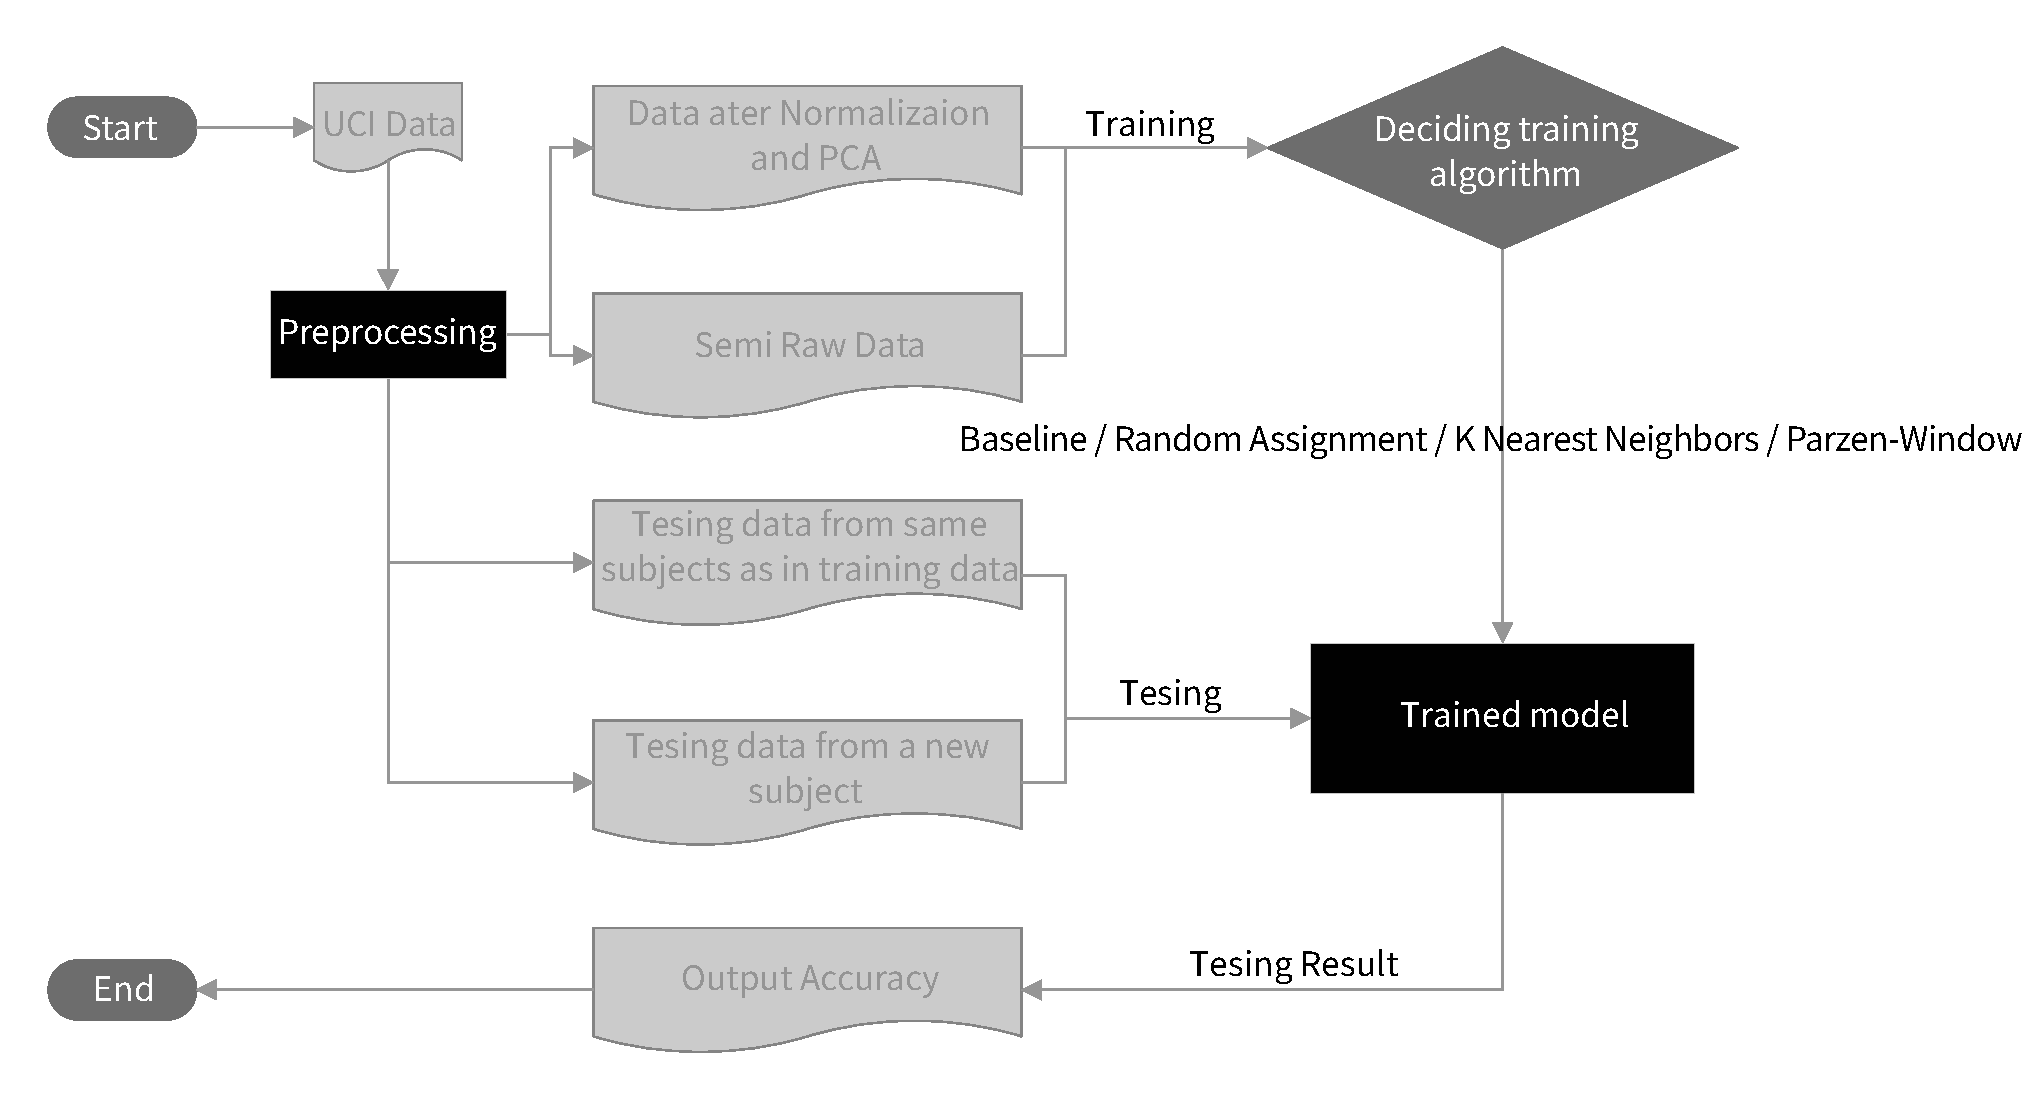
\includegraphics[width=12cm]{workflow.pdf}
}
\end{center}
\caption{Workflow Diagram}
\end{figure}

Other than study the three key components of qualitative activity recognition, we conducted our experiment in a different perspective to explore the breadth of classification algorithms. Our study focuses on analyzing different classification results conducted by different classification models. Our ultimate goal is to be able to distinguish correct activities as well as different wrong activities.

\section{Approach}

\subsection{Data Pre-processing}

Our dataset contains 152 dimensions and 39422 instances. The data pre-processing stage includes transforming categorical data into numerical data, filling and removing sparse data cells, normalizing data, and reducing dimensions. Sparse cells were filled with their corresponding statistical data, such as min, max, mean, and variance. All the numerical data was normalized to have mean zero 0 and covariance 1. Moreover, feature exaction was handled by Principal Component Analysis (PCA) to reduce the dimensions. After we pre-processed the data, the data was reduced to 50 dimensions other than 152.

\subsection{Training Algorithms}

Our training approaches are based on sklearn library written in Python. In this section we will discuss different training algorithms we applied in our project. The following table should provide a general overview about our approaches.

\subsubsection{Random Assignment}

In this approach, we assign a data instance to a random class. Every class has equal probability to be assigned to. Since we have five classes in total, this means every class has 20\% probability to be assigned to. However, as we already know that the distributions of different classes in our data set are different, we do not expect high performance from it. Instead, we will only use it as a benchmark for comparison.

\subsubsection{Random Assignment I}

In our second randomized approach, we also assign a data instance to a class randomly. However, unlike the first random approach, we take the original distribution of different classes in our training data set into considerations. That means different classes have different probabilities to be assigned to. For example, Class 0 is 27.9\% of  training data, therefore, for a testing data instance, it has 27.9\% possibility to be assigned to Class 0. The rest four classes’ possibilities follow the same idea.

\subsubsection{Random Assignment II}

Our third randomized approach is rather simple comparing the previous two. In this approach, we blindly assign all the testing instances to Class 0, which has the highest frequency in the entire data set. Hence, the performance of this approach is within a predictable range. With the test cases we randomly selected for existing subjects, both the semi raw data and the normalized data have 28.63\% accuracy. For new subject, the accuracy rate is 33.56\%.

\subsubsection{Baseline}

In baseline approach, we applied an algorithm which borrows the idea of k nearest neighbour. We use all of our training data to generate five centers of  five classes. For the testing instances, we assignment them to the class with the closest center to them.

\subsubsection{K Nearest Neighbours}

In this training algorithm, we assign a testing instance to a class based on its K nearest neighbours. Among the K nearest neighbours, we find the class, which most of the training instances belong to, then assign the testing instance to that class. In terms of choice of K, we have tried multiple values, among which we found that the square root of total amount of training data gives the best outcome. This specific comes from one of our team members’ previous project experience.

\subsubsection{Parzen-Window}

Parzen-Window approach has very similar idea to K nearest neighbours approach, but also slightly different from it. In parzen-window approach, we focus more on the density of data instances around the testing data. In this case, we exam an area instead of a certain number of neighbours. After we decide the radius of the area we should be looking at, we pick the class that has majority number of instances within that area and assign our testing data to that class. That being said, with different settings of radius R, assignment of classes could be quite different. It is also possible that certain data instance does not have any training data instance within R. Therefore, we will have outliers. In this project and for this approach, we set all outliers to be Class 0, which is the major class in our training data.

\subsubsection{Perceptron and SVM}

In this project, we also included basic machine learning algorithms, such as perceptron and SVM. Since the training phase is based on sklearn package in Python, we used the library’s perceptron and SVM functions. For perceptron, instead of using default 5 times of passes over the training data, we set n\_iter to 1000 and left the rest arguments as default. For SVM, we set the kernel argument as linear instead of the default rbf setting.

\section{Experiments}

\subsection{Tables}

All tables must be centered, neat, clean and legible. Do not use hand-drawn
tables. The table number and title always appear before the table. See
Table~\ref{sample-table}.

Place one line space before the table title, one line space after the table
title, and one line space after the table. The table title must be lower case
(except for first word and proper nouns); tables are numbered consecutively.

\begin{table}[t]
\caption{Sample table title}
\label{sample-table}
\begin{center}
\begin{tabular}{ll}
\multicolumn{1}{c}{\bf PART}  &\multicolumn{1}{c}{\bf DESCRIPTION}
\\ \hline \\
Dendrite         &Input terminal \\
Axon             &Output terminal \\
Soma             &Cell body (contains cell nucleus) \\
\end{tabular}
\end{center}
\end{table}

\section{Conclusion}

Based on our experiment, the maximum accuracy rate we could get for existing subject is 98.30\% and for new subject is 69.45\%, which is really good given the fact that the model does not need any knowledge about the new subject before hand.

In real life scenario, since health is one of the largest focuses in wearable smart device industry, companies like Fitbit or Jawbone could train such a model beforehand and provide their users with further services such as workout quality evaluations and wrong gesture warnings to encourage good exercise as well as to prevent injuries.

\subsubsection*{Contributions}

Wenzhen Gong (\texttt{wenzheng}) implemented the most part of the Python program. Tianhan Zhang (\texttt{tianhanz}) and Dongyuan Liu (\texttt{dla126}) improved the program, fine-tuned the parameters and gathered data. Yan Shi (\texttt{yshi2}) mainly worked on data pre-processing. Each project members participated in choosing the learning algorithms and worked on the project report.

\subsubsection*{References}

\small{
[1] M. Gallagher. Ten most common causes of training injury. {\it Muscle \& Fitness}, June 1996.

[2] Velloso, E.; Bulling, A.; Gellersen, H.; Ugulino, W.; Fuks, H. Qualitative Activity Recognition of Weight Lifting Exercises. {\it Proceedings of 4th International Conference in Cooperation with SIGCHI (Augmented Human `13)}. Stuttgart, Germany: ACM SIGCHI, 2013.
}
\end{document}
